% Copyright (C) 2010,2011 The ESPResSo project
% Copyright (C) 2004 Igor Pasichnyk
% Copyright (C) 2002,2003,2004,2005,2006,2007,2008,2009,2010 Max-Planck-Institute for Polymer Research, Theory Group, PO Box 3148, 55021 Mainz, Germany
%  
% This file is part of ESPResSo.
%   
% ESPResSo is free software: you can redistribute it and/or modify it
% under the terms of the GNU General Public License as published by the
% Free Software Foundation, either version 3 of the License, or (at your
% option) any later version.
%  
% ESPResSo is distributed in the hope that it will be useful, but
% WITHOUT ANY WARRANTY; without even the implied warranty of
% MERCHANTABILITY or FITNESS FOR A PARTICULAR PURPOSE.  See the GNU
% General Public License for more details.
%  
% You should have received a copy of the GNU General Public License
% along with this program.  If not, see <http://www.gnu.org/licenses/>.
%
\documentclass[a4paper, 12pt]{article}
\usepackage[dvips]{graphicx}
\newcommand{\vect}[1]{\mathbf{#1}}
\newcommand{\curl}[1]{\vect{\nabla}\times\vect{#1}}
\newcommand{\diverg}[1]{\vect{\nabla}\cdot\vect{#1}}
\newcommand{\partderiv}[2]{\frac{\partial{#1}}{\partial{#2}}}
\newcommand{\volumeint}{\int d^3\vect r\,}
\def\es{{\sf ESPResSo}}             % Espresso sign
\begin{document}
{\huge{\bf Coulomb Interactions via Local Dynamics: \\
A Molecular--Dynamics Algorithm}}\\
\vspace{0.2cm}
{\bf {\large Igor Pasichnyk\\
Max-Planck-Institut f\"ur Polymerforschung\\
Mainz}}
%
\section{Introduction}
%
The Molecular Dynamics method for obtaining Coulomb interactions as
the potential of mean force between charges which are dynamically
coupled to a local electromagnetic field is described. It is
intimately related to the Car--Parrinello approach, while being
equivalent to solving Maxwell's equations with freely adjustable speed
of light.
%
\section{Equations of motion}
%
Denoting the particle masses with $m_i$, their charges with $q_i$, their coordinates and momentum with $\vect
r_i$ and $\vect p_i$ respectively, the interparticle potential (of {\em non}--electromagnetic
type) with $U$,  for the coupled system of charges and fields we write the following equations of motion
%
\begin{eqnarray} 
  \dot{\vect r}_i & = & \frac{1}{m_i} \vect p_i \\
  \dot{\vect p}_i & = & - \frac{\partial U}{\partial \vect r_i} + q_i \vect E (\vect r_i)- \frac{\zeta}{m_i} \vect p_i
                        + \vect f_i \\
  \dot{\vect A} & = & - \vect E \\
  \dot{\vect E} & = & 
  c^2 \vect \nabla \times \left( \vect \nabla \times \vect A \right)
  - \frac{1}{\epsilon_0} \vect j ,
\end{eqnarray}
%
where $\epsilon_0$ is the vacuum dielectric constant, $c$ speed of light, $\vect A$ the vector-potential, $\vect E$ the elctric field, $\vect j$ the current
density; $\zeta$ is the particle friction constant, and $\vect f_i$ is a
random force satisfying the standard fluctuation--dissipation theorem:
%
\begin{equation}
\left< f_i^\alpha (t) f_j^\beta (t^\prime) \right> =
2 \zeta k_B T \delta_{ij} \delta_{\alpha \beta}
\delta (t - t^\prime),
\end{equation}
%
where $\alpha$ and $\beta$ denote Cartesian indices.

If we introduce the vector $\vect B=\curl A$ the system of equations can be rewritten in a form similar to the usual Maxwell equations. Currently in {\es} the version with $\vect B$ and $\vect E$ is implemented.
%
\section{Discretization}
%
For implementation on the computer, the equations need to be
discretized with respect to both space and time.We consider a domain of physical space as being an
affine space and divide it into subdomains of contiguous cells of
cubic shape. The charges live on the vertices of our lattice which has
the spacing $a$. The electric fields $E(l)$ and vector potentials
$A(l)$ live on the edges or links and are aligned with them. We need
also the operator $\curl{}$. It gives the vector $\vect B$, which lives on the
faces of the cube or on the plaquettes, Fig.~\ref{fig:cell_structure}.
%
\begin{figure}
  \includegraphics[scale=0.55]{figs/cell.eps}
  \caption{Spatial elements of a cell complex}
  \label{fig:cell_structure}  
\end{figure}
%
In the implementation of the algorithm we assume that particles with
masses $m_i$ live in the continuum (off--lattice approach). Particles
have charges $q_i$ and interact between themselves also by a
Lennard--Jones potential. The Lennard--Jones potential of scale $\sigma$ is 
truncated at its minimum, $r_c=2^{1/6}\sigma$. 

The charges are interpolated on the lattice
with grid spacing $a$ using the linear interpolation scheme.
%
\section{Initialization of the algorithm}
%
In order to start the simulation for the given random distribution of
charges we have to calculate the initial electrostatic field, i.~e. the
exact solution of the electrostatic problem. We find a particular solution of Gauss' law as
the result of the following recursive procedure (see
Fig.~\ref{fig:initialization_E}):
\begin{enumerate}
\item The charge in the plane $z=z_{plane}$ is 
\begin{equation}
q_{plane}=\frac{1}{N}\sum_iq(\vect r_i)\delta(z_i-z_{plane}),
\end{equation}
$N$ is the number of charges in plane $z=z_{plane}$. Update the
$z$-field according to the formula
\begin{equation}
E_z^2=E_z^1+\frac{q_{plane}}{\epsilon_0a^2};
\end{equation}
\item Subtract the
charge $q_{plane}$ from the each charge on sites of $z_{plane}$. The
charge of the wire $y=y_{wire}, z=z_{plane}$ is
\begin{equation}
q_{wire}=\frac{1}{N}\sum_iq(\vect r_i)\delta(z_i-z_{plane})\delta(y_i-y_{wire}),
\end{equation}
 $N$ now meaning the
number of charges in the wire. Update $y$-field
\begin{equation}
E_y^2=E_y^1+\frac{q_{wire}}{\epsilon_0a^2};
\end{equation}
\item Subtract the charge $q_{wire}$ from the each charge on the sites of
$(y_{wire},z_{plane})$. Update $x$ field 
\begin{equation}
E_x^2=E_x^1+\frac{q_{vertex}}{\epsilon_0a^2}
\end{equation}
\end{enumerate}

\begin{figure}
 \centering \includegraphics[scale=0.74]{figs/initializationE.eps}
 \caption{Recursive solution of Gauss' law} 
 \label{fig:initialization_E} 
\end{figure} 

%
\section{Time integrator}
%
For the time discretization we have adopted the elegant solution which was found by
Rottler and Maggs \cite{maggs_prl_1} and allows to conserve {\em both}
time--reversibility and phase--space volume conservation:

\begin{enumerate}
\item Update the particle momenta by half a time step.
\item Update the $\vect B$ field by half a time step.
\item Update the particle positions in $x$ direction by half a time step.
\item Update the electric field in $x$ direction by half a time step.
\item Update the particle positions in $y$ direction by half a time step.
\item Update the electric field in $y$ direction by half a time step.
\item Update the particle positions in $z$ direction by half a time step.
\item Update the electric field in $z$ direction by a full time step.
\item Update the particle positions in $z$ direction by half a time step.
\item Update the electric field in $y$ direction by half a time step.
\item Update the particle positions in $y$ direction by half a time step.
\item Update the electric field in $x$ direction by half a time step.
\item Update the particle positions in $x$ direction by half a time step.
\item Update the $\vect B$ field by half a time step.
\item Update the particle momenta by half a time step.
\end{enumerate}
%
\section{Self--energy}
%
The interpolation of the charges onto the lattice gives rise to the
artificial force exerted on the particle by its own field. In order to
cure this remedy, the direct subtraction of the self--energy is introduced.

For the interpolated charge cloud the self--energy can be directly
calculated (see Ref.\cite{phd_pasichnyk}). For the simple cubic
lattice in three dimensions the linear interpolation will give 8
charges which are placed at the corners of the cube with edge length
$a$ (see Fig.~\ref{fig:charge_assig_cubic_lattice}).
%
\begin{figure} 
  \centering \includegraphics[scale=0.55]{figs/charge_assig_cube.eps}
  \caption{Linear interpolation scheme} 
  \label{fig:charge_assig_cubic_lattice}  
\end{figure}
%
Therefore in our case the self-energy is a symmetric bilinear form
defined by the matrix $\left\{\alpha_{ij}\right\}$, the elements of
which do not depend on the position of the charge. In our algorithm
the values of the coefficients
%
\begin{equation}
  \alpha_{ij}=\frac{1}{4a\epsilon_0L^3}\sum\limits_{\vect k}\frac{\cos \vect k(\vect R_{\imath}-\vect R_{\jmath})}{\sum_{\imath=1}^3(1-\cos\vect
      k\vect a_{\imath})}
\end{equation}
%
where $L$ is tne number of lattice points per dimension, $\vect R_i$ coordinates of the interpolated charges and $\vect k$ the wave vector, are calculated during the initialization step and are used in the
calculation of the self-force. The value of the self-force which has
to be subtracted from the overall forces is given by the following
ansatz
%
\begin{equation}
  \vect F_{self}=-\frac{\partial \mathcal U_{self}}{\partial\vect
    r}=-\sum\limits_i\sum\limits_j\alpha_{ij}\left[q_i\frac{\partial
      q_j}{\partial\vect r}+q_j\frac{\partial q_i}{\partial\vect r}\right].
\end{equation}
%
%
\section{Yukawa screening}
%
Rottler and Maggs \cite{maggs_prl_2} suggest another subtraction
scheme which has the nice property of introducing another optimization
parameter $\kappa$ into the method. Essentially, interactions up to
the length scale $\kappa^{-1}$ are done in real space, while only the
residual long--range part beyond $\kappa^{-1}$ is treated via the
dynamics. A scalar field $\phi$ that couples to the interpolated charges via the energy functional
%
\begin{equation}
{\cal F}\left[\phi\right]= \frac{\epsilon_0}{2} \int d^3 \vect r\left( \vect{\nabla} \phi \right)^2
+ \frac{\epsilon_0}{2} \int d^3 \vect r \kappa^2 \phi^2 + \int d^3 \vect r \, \rho \phi
\end{equation}
%
where $\rho$ is the charge density, leads to an effective interaction between particles of the form
%
\begin{equation}
  U_Y(\vect r)=-\frac{q_iq_j}{4\pi\epsilon_0 r}exp(-\kappa r)
\end{equation}
%
In the algorithm the field $\phi$ obeys the equation of motion
%
\begin{equation}
  \frac{1}{c_{\phi}^2}\frac{\partial^2\phi}{\partial t^2}=\nabla^2\phi-\kappa\phi-\rho
\end{equation}
%
where $c_{\phi}$ is another dynamical parameter of dimension velocity. Currently $c_{\phi}$ is equal to the speed of light. 

In our algorithm we use Yukawa screening to resolve interparticle
interactions on a local scale, such that larger spacings are
feasible. In the method we subtract the self-energy for both the
screened and the unscreened interaction separately by the respective
exact lattice Green's function.  Finally, the Yukawa potential is
corrected at short distances by adding an extra analytic Yukawa
potential (with opposite sign) to the truncated Lennard--Jones
potential.

\begin{thebibliography}{10}

\bibitem{maggs_prl_1}
Rottler J and Maggs A~C \emph{Local molecular dynamics with coulombic
  interaction} cond-mat/0312438
\bibitem{phd_pasichnyk}
Pasichnyk I \emph{Novel simulation methods for Coulomb and hydrodynamic interactions}, PhD thesis, Mainz, 2004
\bibitem{maggs_prl_2}
Rottler J and Maggs A~C \emph{A Continuum, {$\cal O(N)$} Monte-Carlo algorithm for charged particles}, Journal of Chemical Physics, 120, 3119-3129, 2004
\bibitem{espressowebsite}
See web site \url{http://espressomd.org}
\end{thebibliography}

\end{document}
